\chapter{Facade模式}
\section{Facade模式的概念}
\subsection{外观模式的定义}
外观(Facade)模式的定义:是一种通过为多个复杂的子系统提供一个一致的接口,而使这些子系统更加容易被访问的模式。该模式对外有一个统一接口,外部应用程序不用关心内部子系统的具体的细节,这样会大大降低应用程序的复杂度,提高了程序的可维护性。
\subsection{特点}
\begin{enumerate}
	\item 降低了子系统与客户端之间的耦合度,使得子系统的变化不会影响调用它的客户类。
	\item 对客户屏蔽了子系统组件,减少了客户处理的对象数目,并使得子系统使用起来更加容易。
	\item 降低了大型软件系统中的编译依赖性,简化了系统在不同平台之间的移植过程,因为编译一个子系统不会影响其他的子系统,也不会影响外观对象。
\end{enumerate}
\subsection{缺点}
\begin{enumerate}
	\item 不能很好地限制客户使用子系统类。
	\item 增加新的子系统可能需要修改外观类或客户端的源代码,违背了“开闭原则”。
\end{enumerate}
\subsection{应用场景}
\begin{enumerate}
	\item 对分层结构系统构建时,使用外观模式定义子系统中每层的入口点可以简化子系统之间的依赖关系。
	\item 当一个复杂系统的子系统很多时,外观模式可以为系统设计一个简单的接口供外界访问。
	\item 当客户端与多个子系统之间存在很大的联系时,引入外观模式可将它们分离,从而提高子系统的独立性和可移植性。
\end{enumerate}
注:
\par 外观模式可以为互相关联在一起的错综复杂的类整理出高层接口,其中Facade角色
可以让系统对外只有一个简单的接口,Facade角色还会考虑到系统内部各个类之间的
责任关系和依赖关系,按照正确顺序调用各个类。
\subsection{外观模式的角色}
\begin{enumerate}
	\item Facade外观:为多个子系统对外提供一个共同的接口;
	\item Subsystem子系统:实现系统的部分功能,客户可以通过外观角色访问它;
	\item Client请求者:通过一个外观角色访问各个子系统的功能。
\end{enumerate}
\section{外观模式实现——例一}
\begin{table}[!h]
	\begin{tabular}{|l|l|l|}
		\hline
		包&名字&说明\\
		\hline
		pagemaker&Database&从邮件地址获取用户名的类\\
		\hline
		pagemaker&HtmlWriter&编写HTML文件的类\\
		\hline
		pagemaker&PageMaker&根据邮件地址编写该用户的Web页面\\
		\hline
		&Main&测试程序行为\\
		\hline
	\end{tabular}
\end{table}
\begin{figure}[!h]
	\centering
	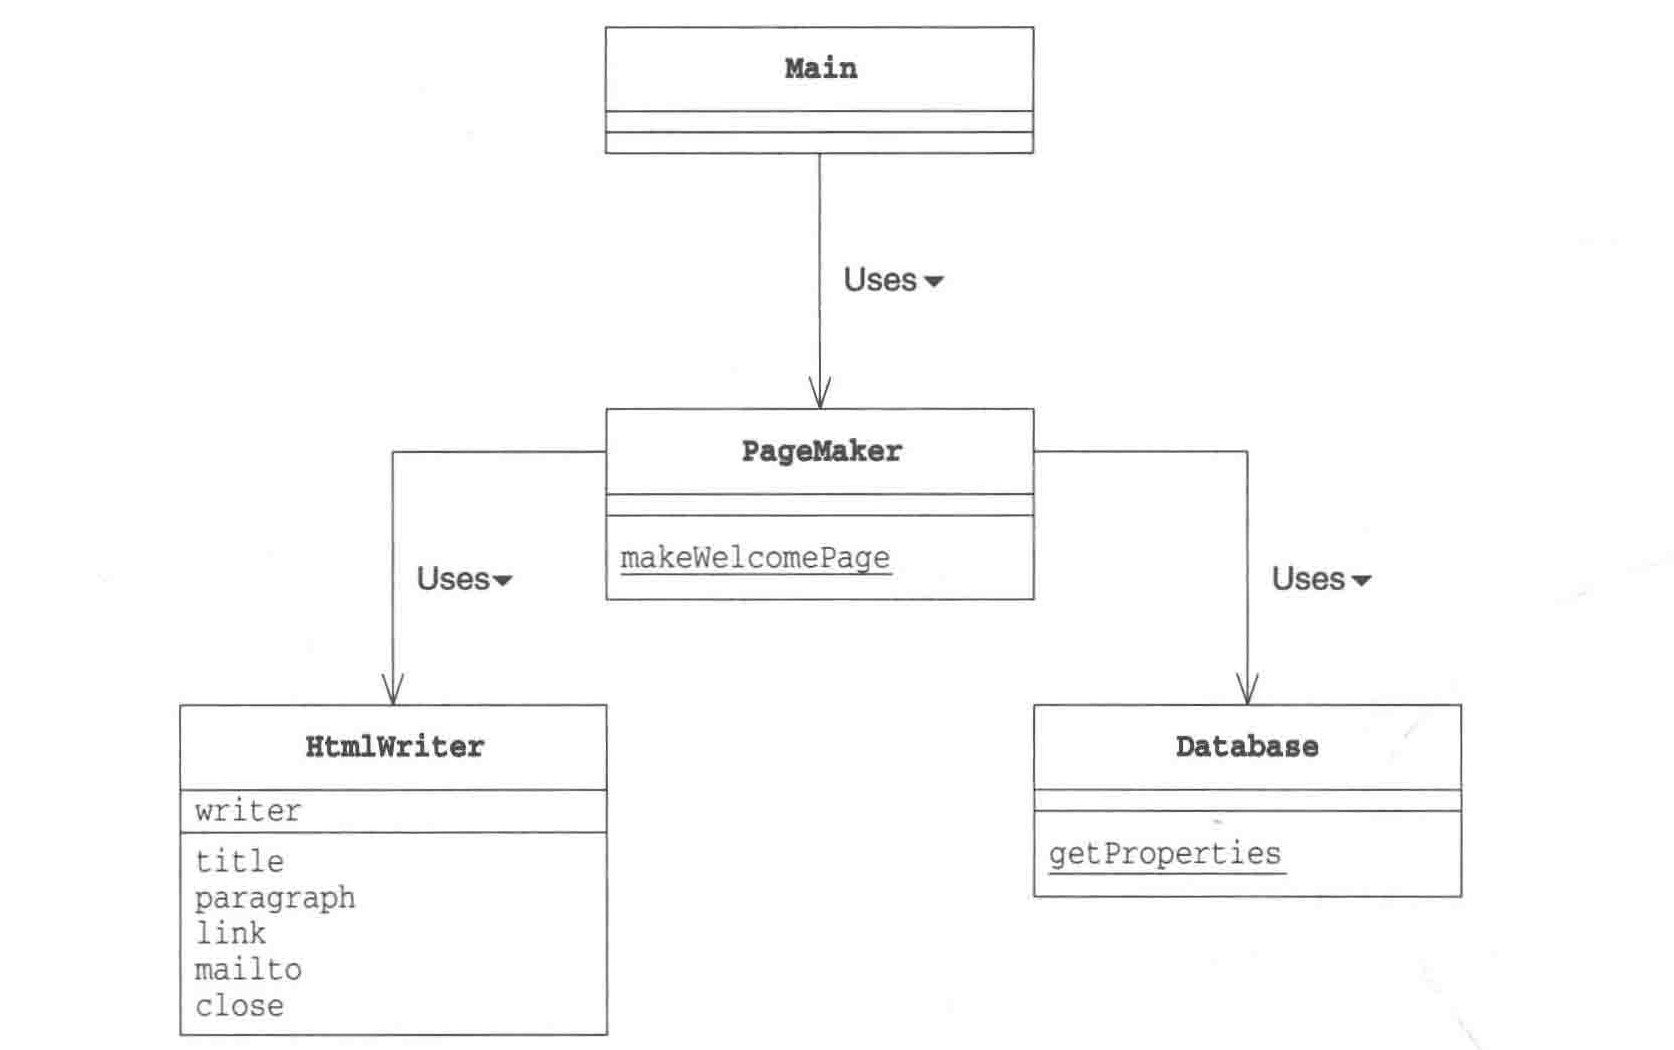
\includegraphics[width=\textwidth]{image/15-3}
	\caption{外观模式的类图}
\end{figure}
\begin{lstlisting}
public class DataBase {
	private DataBase() {}
	//根据数据库名获取 properties
	public static Properties getProperties(String dbName) {
		String fileName = dbName + ".txt";
		Properties prop = new Properties();
		try {
			prop.load(new FileInputStream(fileName));
		} catch (IOException e) {
			System.out.println("Warning: " + fileName + " is not found.");
		}
		return prop;
	}
}
\end{lstlisting}
\begin{lstlisting}
//文件maildata.txt
hyuki@hyuki.com=Hiroshi Yuki
hanako@hyuki.com=Hanako Sato
tomura@hyuki.com=Tomura
mamoru@hyuki.com=Mamoru Takahashi
\end{lstlisting}
\begin{lstlisting}
//编写简单的 Web 页面
public class HtmlWriter {
	private Writer writer;
	public HtmlWriter(Writer writer) {
		this.writer = writer;
	}
	public void title(String title) throws IOException {
		writer.write("<html>");
		writer.write("<head>");
		writer.write("<title>" + title + "</title>");
		writer.write("</head>");
		writer.write("<body>\n");
		writer.write("<h1>" + title + "</h1>\n");
	}
	public void paragraph(String msg) throws IOException {
		writer.write("<p>" + msg + "</p>\n");
	}
	public void link(String href, String caption) throws IOException {
		paragraph("<a href=\"" + href + "\">" + caption + "</a>");
	}
	public void mailto(String mailaddr, String userName) throws IOException {
		link("mailto:" + mailaddr, userName);
	}
	public void close() throws IOException {
		writer.write("</body>");
		writer.write("</html>\n");
		writer.close();
	}
}
\end{lstlisting}
\begin{lstlisting}
//使用 DataBase 和 HtmlWriter 生成指定用户的页面
public class PageMaker {
	private PageMaker() {}
	public static void makeWelcomePage(String mailaddr, String fileName) {
		try {
			Properties mailProp = DataBase.getProperties("maildata");
			String userName = mailProp.getProperty(mailaddr);
			HtmlWriter writer = new HtmlWriter(new FileWriter(fileName));
			writer.title("Welcome to " + userName + "'s page!");
			writer.paragraph(userName + "欢迎来到" + userName + "的主页");
			writer.paragraph("等着你的邮件喔!");
			writer.mailto(mailaddr, userName);
			writer.close();
			System.out.println(fileName + " is created for " + mailaddr + " (" + userName + ")");
		} catch (IOException e) {
			e.printStackTrace();
		}
	}
}
\end{lstlisting}
\begin{lstlisting}
public class Main {
	public static void main(String[] args) {
		PageMaker.makeWelcomePage("hyuki@hyuki.com", "welcome.html");
	}
}
\end{lstlisting}
\section{外观模式实现——例二}
\begin{figure}[!h]
	\centering
	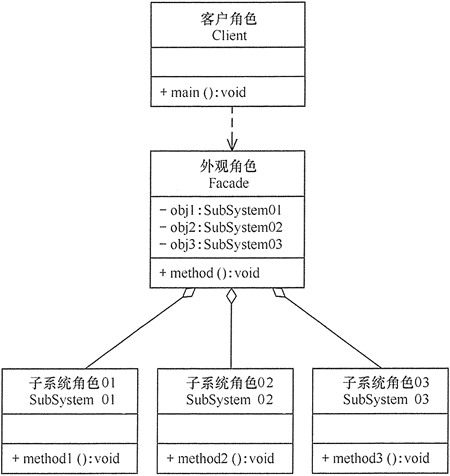
\includegraphics[width=0.6\textwidth]{image/15-1}
	\caption{外观模式的结构图}
\end{figure}
\begin{lstlisting}
//外观角色
class Facade {
	private SubSystem01 obj1 = new SubSystem01();
	private SubSystem02 obj2 = new SubSystem02();
	private SubSystem03 obj3 = new SubSystem03();
	
	public void method() {
		obj1.method1();
		obj2.method2();
		obj3.method3();
	}
}
\end{lstlisting}
\begin{lstlisting}
//子系统角色
class SubSystem01 {
	public void method1() {
		System.out.println("子系统01的method1()被调用!");
	}
}

//子系统角色
class SubSystem02 {
	public void method2() {
		System.out.println("子系统02的method2()被调用!");
	}
}

//子系统角色
class SubSystem03 {
	public void method3() {
		System.out.println("子系统03的method3()被调用!");
	}
}
\end{lstlisting}
\begin{lstlisting}
public class FacadePattern {
	public static void main(String[] args) {
		Facade f = new Facade();
		f.method();
	}
}
\end{lstlisting}
\section{扩展模式}
在外观模式中,当增加或移除子系统时需要修改外观类,这违背了“开闭原则”。如果引入抽象外观类,则在一定程度上解决了该问题,如下图:
\begin{figure}[!h]
	\centering
	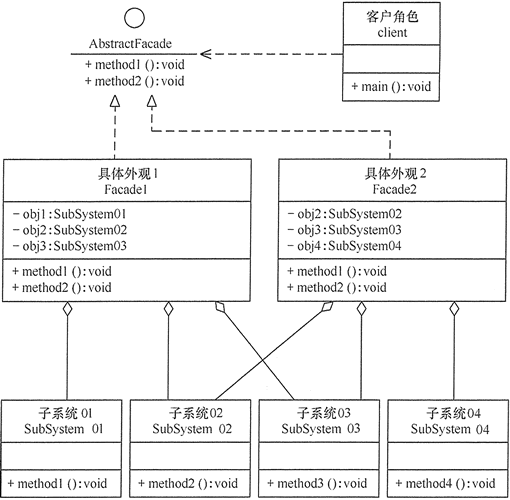
\includegraphics[width=0.8\textwidth]{image/15-2}
	\caption{引入抽象外观类的外观模式的结构图}
\end{figure}
\section{扩展思路}
\begin{enumerate}
	\item Facade的工作:使得接口API变少,程序与外部关联关系弱化,另外如果public方法过多,
	会导致类的内部修改变得困难(如果公开,其他类也会读取会使用该public)。
	\item 递归地使用Facade,针对持有几个Facade角色的类的集合。
\end{enumerate}
\section{相关设计模式}
\begin{enumerate}
	\item Abstract Factory可以看做生成复杂实例时的Facade。
	\item 有时使用Singleton创建Facade。
	\item Mediator中,Mediator角色作为Colleague角色的仲裁者或负责调停,Facade中Facade角色
	单方面使用其他角色来提供高层接口,Facade是单向的,Mediator是双向的。
\end{enumerate}